\section{Trigger Hardware and Software}

\par
The Hall A trigger was designed by the
University of New Hampshire.
Here we give a brief overview of the 
hardware arrangement,
the logic of the trigger, and the usage
of the software control.
Diagrams of the hardware layout are shown in
three accompanying 
figures for the E-arm, H-arm,
and coincidence circuit.

\par
Scintillators make the main, so-called S-Ray,
trigger in each spectrometer arm, and a
coincidence is formed between the spectrometer
arms.  The S-Ray trigger is formed by
requiring that scintillator paddles in
planes S1 and S2 both fired (and both phototubes
in each paddle), and that the paddle
combinations in S1 and S2 belong to an
allowed set.  A memory lookup (MLU) decides
if the combination is valid.  The allowed
combinations are for ``S-Ray'' tracks that are at
an approximately 45 degree angle with respect
to the hall floor, with a tolerance of $\pm$1
paddle on either S1 or S2.  The timing of
this trigger is determined by a strobe on
the MLU which in most events comes from the 
right-side PMTs of the S2 plane.  The coincidence
is formed in an overlap AND circuit with
a 110 nsec window.  The electron arm singles
triggers are called T1 (event type 1) in CODA,
the hadron arm singles are T3, and the coincidences
are T5.  If T1 doesn't exist, a looser trigger
called T2 is considered (similarly for T3/T4 on
H-arm).  This looser trigger requires any hit
in 2 out of the following 3 detectors: 
S1,S2, and Cerenkov
(in the case that a Cerenkov detector is used), 
or 1 out of 2 from S1 and S2 if there is no
Cerenkov detector in the spectrometer.  
These looser triggers are prescaled,
and a sample of about 5 Hz from them allows for
an accurate measurement of inefficiencies.
The trigger design is quite flexible and it
is relatively easy to add detectors to define
new trigger types or to modify existing ones,
so long as the detector is fast enough.
The trigger supervisor also allows for the
possibility of 2nd level triggers which could
be used for a later decision.

\begin{figure}
\begin{center}
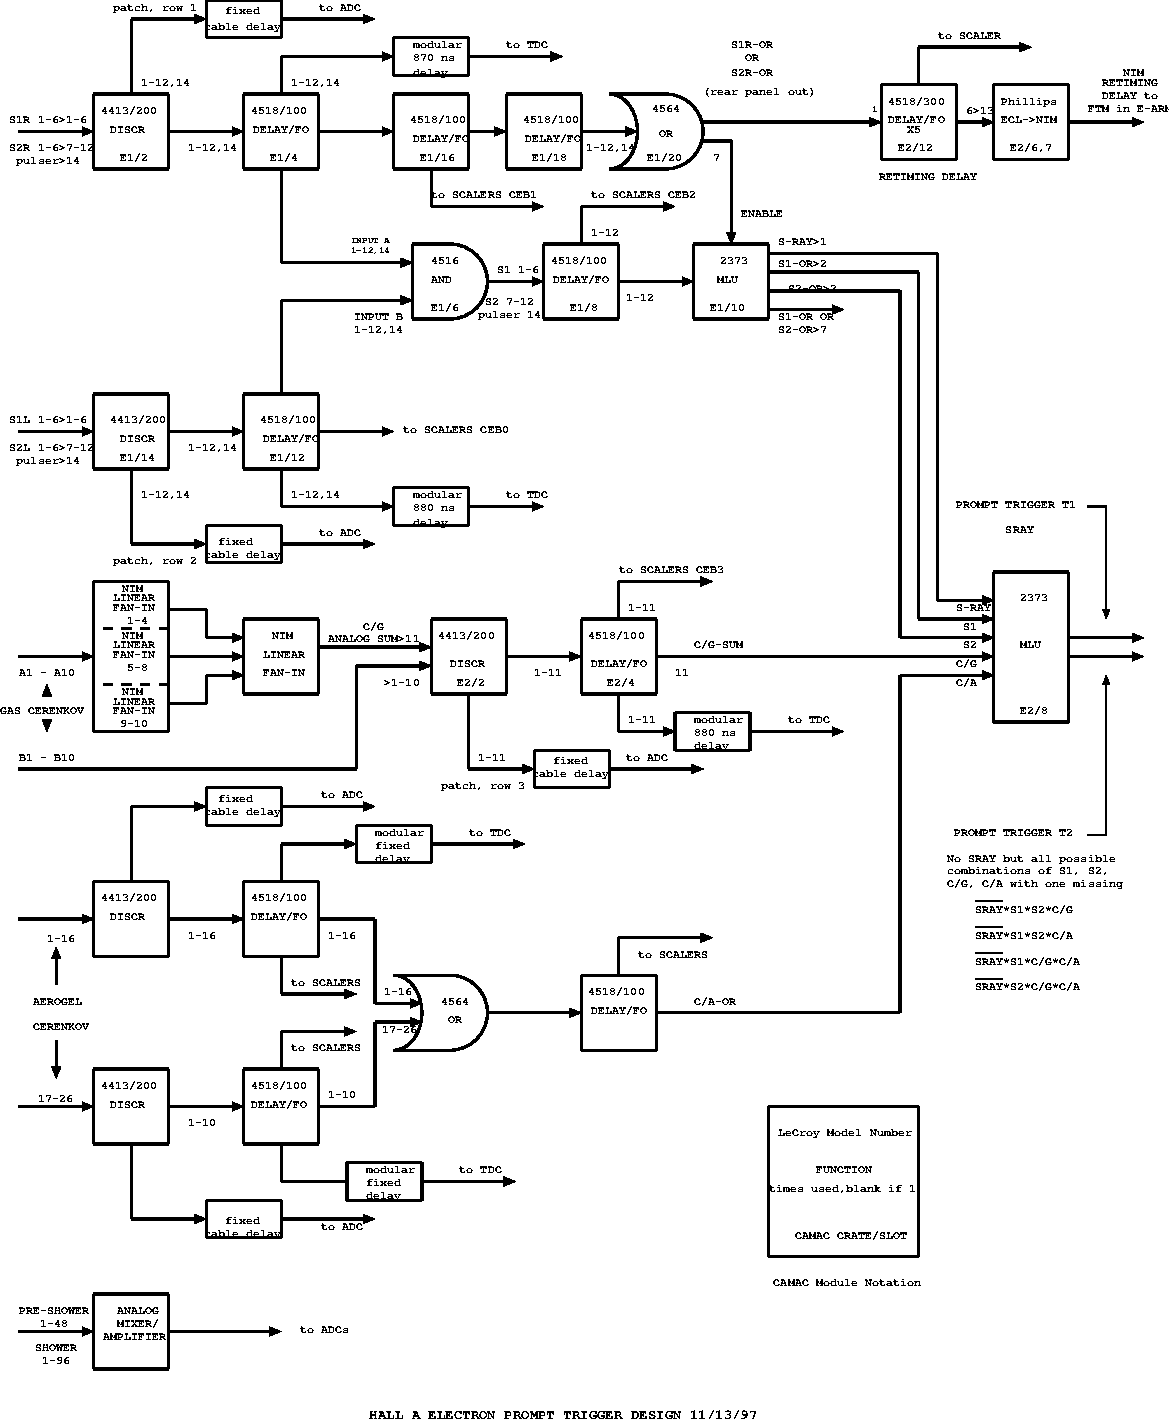
\includegraphics[angle=0,width=15cm,clip]{etrig}
{\linespread{1.}
\caption[Data Acquisition: Electron Arm Trigger]{Electron Arm Trigger Circuit.}
\label{fig:etrig}}
\end{center}
\end{figure}

\begin{figure}
\begin{center}
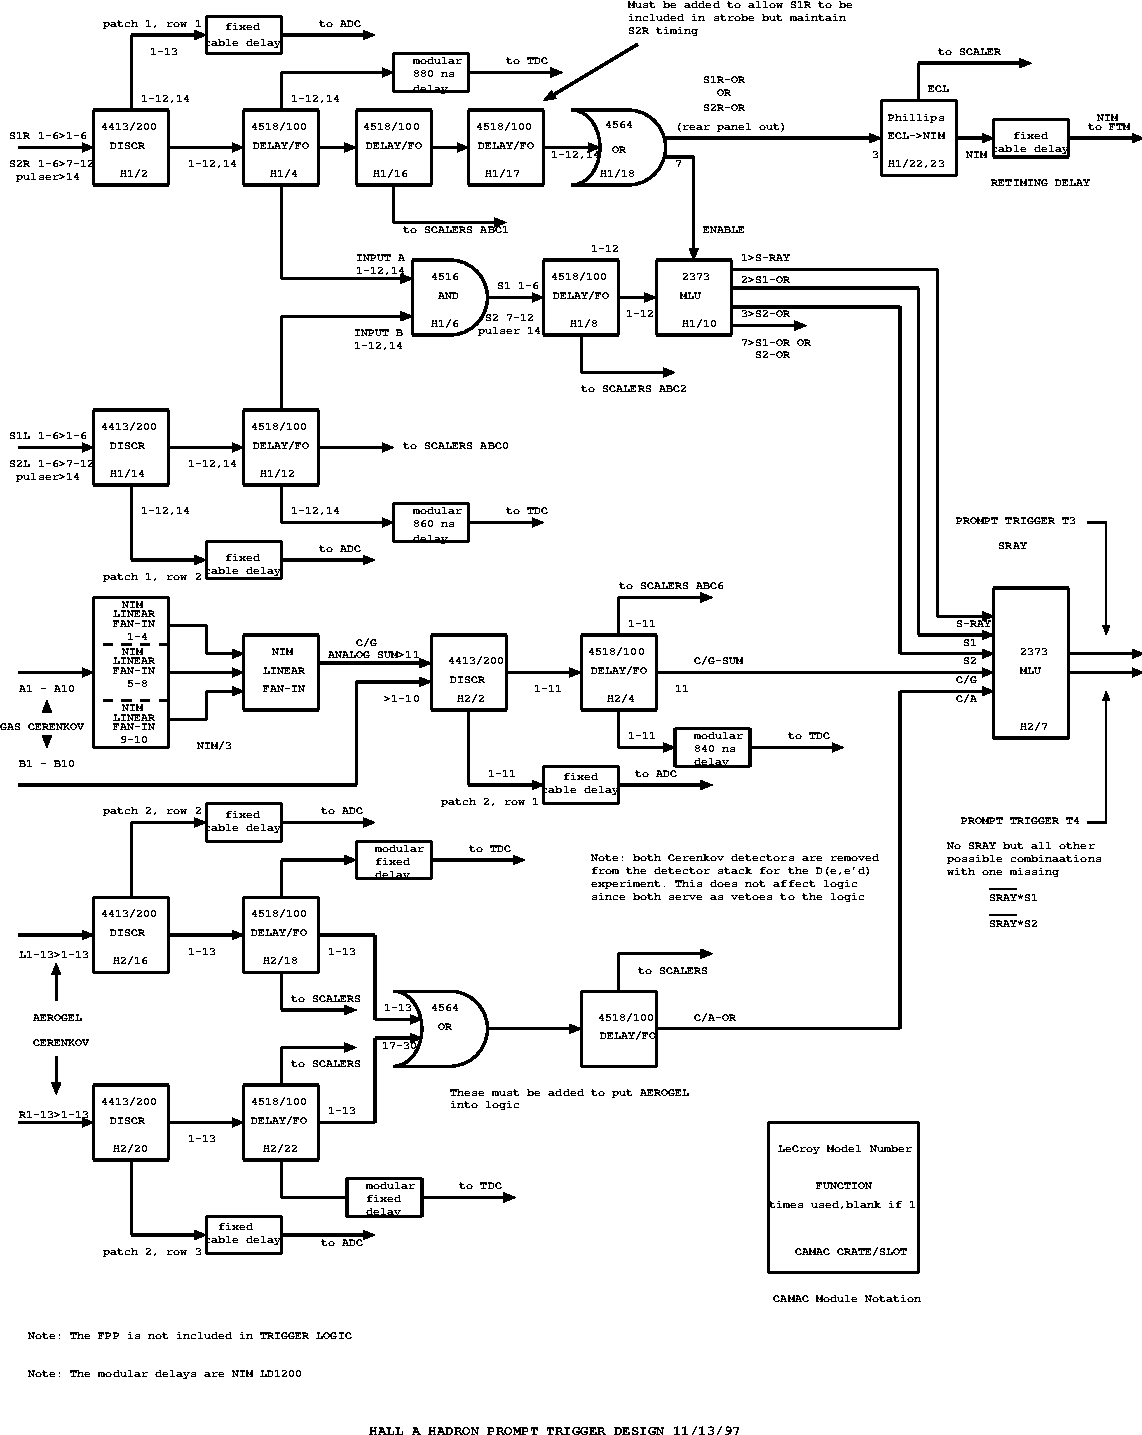
\includegraphics[angle=0,width=15cm,clip]{htrig}
{\linespread{1.}
\caption[Data Acquisition: Hadron Arm Trigger]{Hadron Arm Trigger Circuit.}
\label{fig:htrig}}
\end{center}
\end{figure}

\begin{figure}
\begin{center}
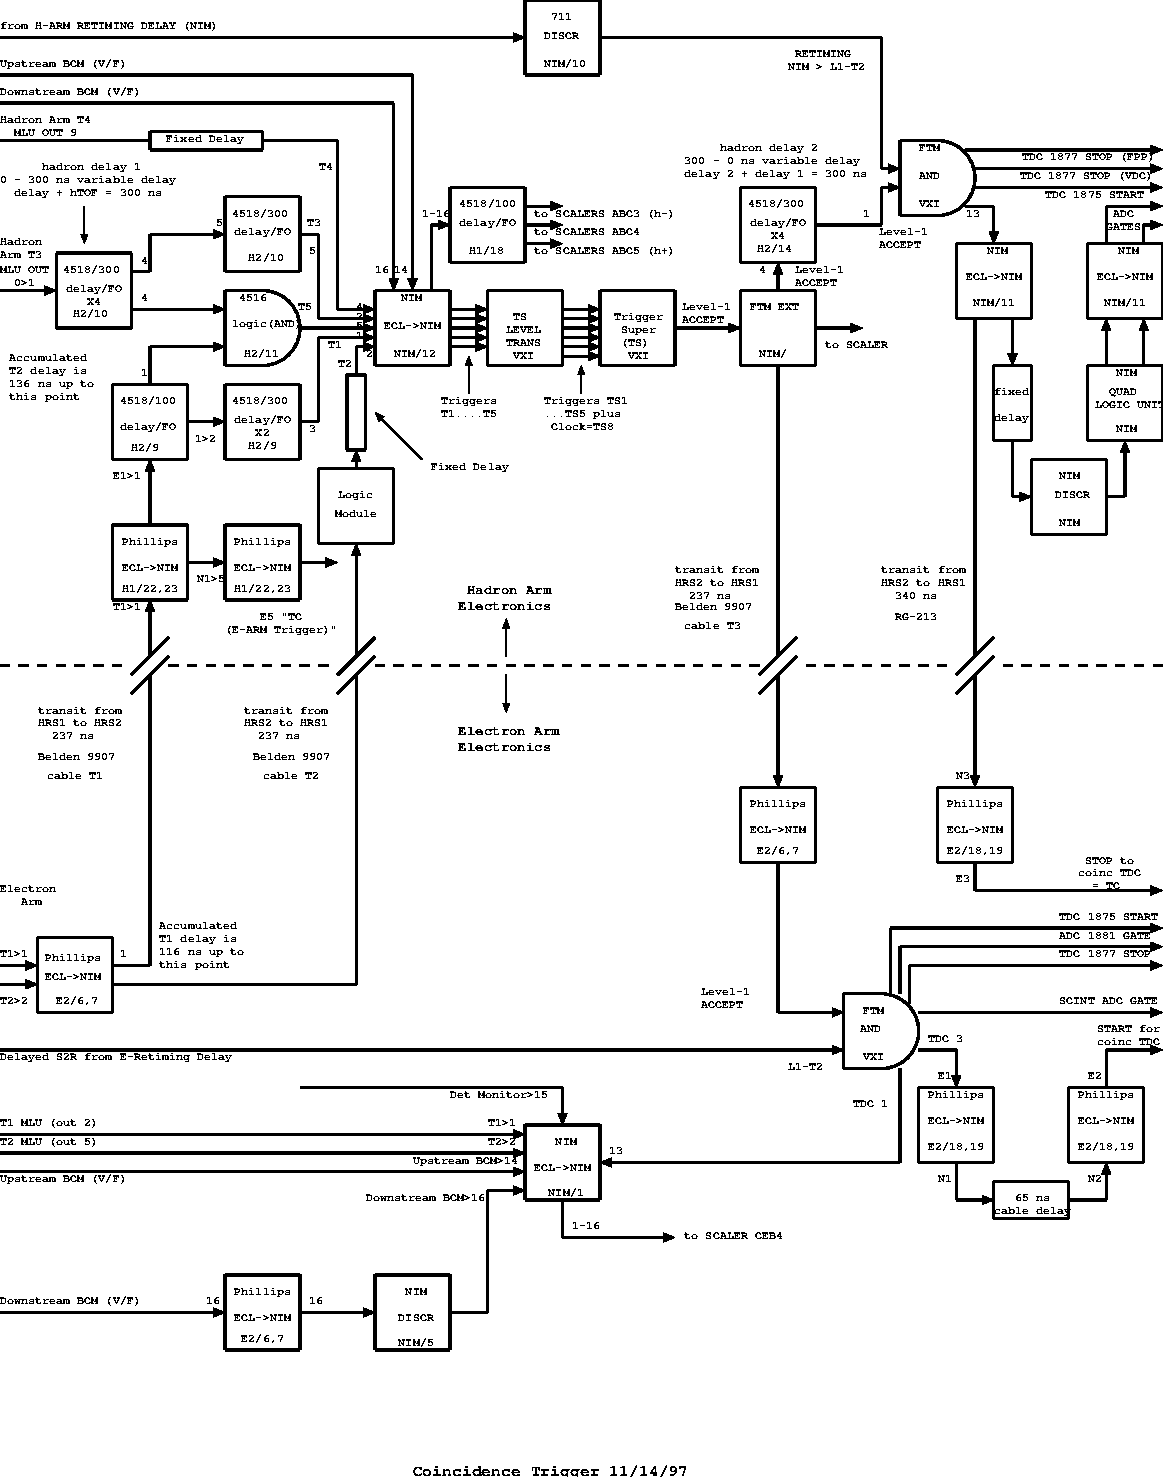
\includegraphics[angle=0,width=15cm,clip]{coinc}
{\linespread{1.}
\caption[Data Acquisition: Coincidence Trigger]{Coincidence Trigger Circuit.}
\label{fig:ctrig}}
\end{center}
\end{figure}

\par
Here we describe the software control
of the CAMAC modules involved in the trigger.
There are four types of modules that
are controlled:
\hskip 0.05in 
1) Discriminators;
\hskip 0.05in 
2) Delay Units;
\hskip 0.05in 
3) Memory Lookup Unit
\hskip 0.05in 
4) AND/OR Modules
\hskip 0.05in 
A graphical user interface called
XTrigMang was written by
T. Smith (UNH).  
XTrigMang is used to download
the trigger and read back values.
This GUI reads in a default setup file and
with one button, called ``Download All'',
one may load the default setup.
To start XTrigMang, login to adaqh2 as
the ``adaq'' account, then type ``gotrigger''
to go to the correct directory (which
contains the default setup in trigsetup.settings), 
and type ``XTrigMang'' there.
For experiments that never change
the trigger, one only needs to ``Download All''
to ensure the trigger is set up after
power is turned on for the crates.
For coincidence experiments it is anticipated
that the only change one needs to make is the
delay on the hadron arm to accommodate
momentum changes.  
Proton momenta above 360 MeV/c are at
present accommodated by the hardware (it would
be a fairly easy hardware change to go lower).
For coincidence experiments, instead
of using XTrigMang directly, one must download
the trigger with a script called trigsetup.
Login to adaqh2 as ``adaq'' account and
type ``trigsetup''.  It asks for the 
momentum of the H-arm (under the assumption
that a proton is in the H-arm and that the E-arm has
an electron with respect to which the H-arm must be
delayed).  Then trigsetup loads the
correct default setup file and starts
XTrigMang, which pops up.  At this point, 
you simply press
the ``Download All'' button in XTrigMang
to setup the trigger.  


\par
If individual modules need to be modified
for test purposes etc. (e.g. to change thresholds),
one may press on the buttons in the XTrigMang
GUI and pop up the components in an obvious way.
Each component has four buttons which it is
essential to understand: 
\hskip 0.05in
1) The ``Set'' button.  One must enter the choice
and then press ``Set''.  This loads your choice
into memory on the workstation ({\it not} on 
the CAMAC crate).
\hskip 0.05in
2) The ``Down'' button.  This sends whatever choice
is in memory to the CAMAC crate.
\hskip 0.05in
3) The ``Show'' button.  This reads back from CAMAC
what is actually in the module.
\hskip 0.05in
4) The ``Read'' button.  This shows what is in
memory on your workstation.  Note that ``read'' is quite 
different from ``show''.
A typical operation to modify a trigger module
would be to Set the value,
Download it, and then Show to check that the value
is in the CAMAC module.  

% ===========  CVS info
% $Header: /group/halla/analysis/cvs/tex/osp/src/daq_trig/trigger.tex,v 1.2 2003/06/05 23:30:00 gen Exp $
% $Id: trigger.tex,v 1.2 2003/06/05 23:30:00 gen Exp $
% $Author: gen $
% $Date: 2003/06/05 23:30:00 $
% $Name:  $
% $Locker:  $
% $Log: trigger.tex,v $
% Revision 1.2  2003/06/05 23:30:00  gen
% Revision ID is printed in TeX
%
% Revision 1.1.1.1  2003/06/05 17:28:32  gen
% Imported from /home/gen/tex/OSP
%
%  Revision parameters to appear on the output
{\small
\begin{verbatim}CVS $Id: trigger.tex,v 1.2 2003/06/05 23:30:00 gen Exp $\end{verbatim}
}
